\documentclass[letterpaper,10pt]{article}
\usepackage{texdraw}
\usepackage{graphicx}
\usepackage{epsf}
%\usepackage{setspace}
\usepackage{array}
\usepackage{paralist}
\usepackage{cite}
\usepackage{enumitem}
\usepackage{subfigure}
\usepackage{color,graphicx,amssymb,amsmath}
\usepackage{verbatim}
\usepackage{setspace}
\sloppy
\usepackage{geometry}
%\usepackage{endfloat}


%%%%%%%% COMPRESS %%%%%%
\usepackage[small,compact]{titlesec}
\usepackage{times}
\setlength{\parindent}{0in}
\setlength{\parskip}{5pt}
\setlength{\floatsep}{5pt}
\setlength{\textfloatsep}{5pt}
\setlength{\intextsep}{2pt}
\setlength{\abovecaptionskip}{2pt}
\setlength{\belowcaptionskip}{2pt}
%lists
\setlength{\topsep}{5pt}
\setlength{\itemsep}{5pt}	
%%%%%%%%  COMPRESS %%%%%%%

%\renewcommand{\figureplace}{%
%      \begin{center}
%      [\figurename~\thepostfig\ ]
%      \end{center}
%   }
%   \renewcommand{\tableplace}{%
%     \begin{center}
%      [\tablename~\theposttbl\ ]
%      \end{center}
% }

%%\renewcommand{\efloatseparator}{\mbox{}}
%\renewcommand{\efloatseparator}{\vspace{20pt}}

% When the final version is ready, replace the definition:
\newcommand{\mycomment}[1]{{\textcolor{red}{\bf {#1}}}}
% by the definition:
%\newcommand{\mycomment}[1]{}
% just to be sure that there are no comments remaining.

\setlength{\leftmargin}{0pt}
\setlength{\listparindent}{0pt}
\oddsidemargin -.025in 
\evensidemargin -0.025in 
%\textwidth 6.75in 
\textwidth 6.5in 
\headheight 0.0in 
\topmargin -0.25in 
%\textheight 10.0in
\textheight 9.0in 

\let\thebibliographyOLD\thebibliography
\renewcommand{\thebibliography}[1]{\thebibliographyOLD{#1}\setlength{\itemsep}{-1mm}}

\begin{document}

\title{}
\author{}
\maketitle

\section{Introduction}

% $Header: /projects/VU-SAGA/Papers/saga_engine_2006/intro.tex,v 1.8 2006/08/13 18:01:00 hkaiser Exp $

  % Grid computing is commonly defined as distributed computing with a
  % focus on highly dynamic environments~\cite{CS_Foster01a,
  % CS_Foster02a}: any application running in grids therefore must be
  % aware of the volatile and dynamic nature of the environment. 
  The Simple API for Grid Applications (SAGA) is one of the most
  prominent recent developments allowing to make it easier to write
  applications leveraging the possibilities of grids, even for
  scientists having no background in computer science, or grid computing.
  
  The presented C++ implementation of the SAGA API is supposed to be
  used as a reference implementation during the OGF standardization
  process. It has a number of key features, which are described later
  in the text in more detail:

  \begin{itemize}
     
    \item Synchronous, asynchronous and task oriented versions of every
    operation are transparently provided.

    \item Dynamically loaded adaptors bind the API to the respective
    grid middleware environment, on runtime, but static pre-binding at link
    time is also supported.
          
    \item Adaptors are selected on a call-by-call basis (late
    binding), allowing for incomplete adaptors, and inherent fail
    safety. A generic object state repository supports the late binding.
    
    \item Latency hiding schemes such as asynchronous operations and bulk
    optimizations are generically and transparently integrated, even
    if not explicitly supported by the adaptors or the respective middleware.

		\item A modular API architecture allows to minimize the runtime 
		memory footprint.
		
    \item API extensions are greatly simplified by the encapsulation of a
    generic call routing mechanism, and by macros resembling the 
    Scientific Interface Description Language (SIDL) used in the 
    SAGA specification. 
    
    \item Strict adherence to Standard-C++ and the utilization of 
    Boost~\cite{boost_website} allows for excellent portability 
    and platform independence.

  \end{itemize}

  The remainder of the paper is structured as follows: the next
  section lists the main design objectives for our implementation.
  The realization of these objectives is then described in the
  following sections, including a more detailed description of the key
  features listed above.  We conclude with some observations we hope
  are useful for other API implementers, and shortly describe our
  future plans.
 




\section{Results From Prior Awards}

Previously we have used TeraGrid resources to conduct a binding affinity study of the protease inhibitor saquinavir with G48V and L90M containing mutatants which showed good agreement with experiment \cite{Stoica2008}. % uring SuperComputing 2007 we used
Using Lonestar (TG allocation number TG-ASC070019T) to expand this work by running 10ns-long simulations on 5 different HIV protease systems bound to 5 different FDA-approved drugs: amprenavir, indinavir, lopinavir, ritonavir, and saquinavir. We compared our binding energy results for each of the 5 protease genotypes in the MDR set to experimental values published in \cite{Ohtaka2003}. Our results showed varying correlations to experimental trends, with the 5 ritonavir systems showing good correlation to experimental whilst the 5 saquinavir systems showed poor correlation. In light of these results further work was done both on Lonestar (TG allocation numbers TG-ASC070019T and TG-DMR070014N) and more recently Ranger (TG allocation numbers A-rfUser1 and TG-ASC090009) to determine whether repeating the study as an ensemble of MD models would improve correlations. The results showed significantly improved correlations and have led us to refine our simulation protocol and reparameterise a number of inhibitors. An article focussed primarily on our work on the lopinavir bound system has recently been accepted for publication \cite{Sadiq2010}.

In addition to this we have performed a study into the comparative dynamics of different liganded forms of reverse transcriptase, concluding that the binding of the inhibitors efavirenz and nevirapine alter the motions of the catalytically important fingers domain of RT and that these motions are uncorrelated to fluctuations in the drug binding energy (as yet unpublished). We also performed preliminary investigations into the efficacy of the ensemble methodology for calculating binding affinities on NVP bound systems, again concluding that the convergence properties are improved over single trajectory. These results also allowed us to differentiate binding affinity of the L100I and L100I/K103N sequences from the wildtype using simulations of the ligand bound enzyme alone which indicates that they do not significantly affect the creation of the binding pocket. All this work was performed using Ranger. 

These simulations were orchestrated using our automated simulation tool, the Binding Affinity Calculator (BAC), which makes use of AHE \cite{coveney2007,zasada2009} to deploy and run simulations and then retrieve data. Two papers describing this tool and its potential use as a clinical support tool have been published\cite{Sadiq2008, Sadiq2008a}. The BAC allows us to distribute the simulation and analysis sections of our workflow over a number of geographically disparate locations. The mutation and hydration of crystal structure based models takes place on local resources at UCL, using the AMBER software suite, while the actual simulations can be performed in NAMD either on TeraGrid or UKNational Grid Service (NGS) computers and/or EU DEISA grid. The final analysis of the resultant trajectories, either on local recources or the NGS, is performed using the AMBER MD suite of codes. In the last year, BAC has been extended to allow the simulation of the epidermal growth factor receptor (EGFR) and the molecular dynamics code GROMACS \cite{Hess2008}. This new functionality has facilitated a study of the binding of three inhibitors (AEE788, AFN941 and getfitinib) bound to EGFR, performed on Ranger.

In the area of bio-minerals our previous simulations have utilized periodic boundaries on the clay sheets, allowing a simulation cell to represent an infinite clay platelet \cite{JPCC_2007,Thyveetil,Thyveetil_JACS, Soft_Matter1}. These large-scale, fully atomistic simulations, approached the size of a physically realistic platelet. From this, we were able to calculate mesoscopic and macroscopic properties directly from molecular dynamics simulations in the absence of finite-size effects of both clay nanocomposites\cite{JPCC_2007,Thyveetil, Soft_Matter1} and bio-composites~\cite{Thyveetil_JACS}.  Using resources from TG-ASC070019T we extended these simulations to calculate the mechanical response of poly(ethylene oxide) polymer-clay nanocomposites, separating the response into contributions from the polymer and clay mineral layer~\cite{Soft_Matter1}. This separation technique allowed us to determine how the clay-polymer elastic properties change with distance from the clay surface. This is the first time the effect of mineral layers on the elastic modulus of polymeric materials in the vicinity of a mineral surface has been calculated. This result is a vital first step to understanding the enhancement mechanism of nanocomposites and the role of the very large surface area of the clay mineral layer on the surrounding medium.  We have also examined the mechanisms by which clay mineral layers buckle in clay-polymer nanocomposites under compressive stress. We find that a clay sheet remains stable in a flat state until a critical compressive strain is reached, at which point it buckles, and regains its uncompressed area. Over this buckling transition, the Poisson ratio of the clay sheets turns negative, a property which has been predicted for 2-dimensional sheets ~\cite{Soft_Matter2}. This is the first time such behaviour has been seen in a molecular simulation of mineral layers. The large scale allowing us to probe large buckling wavelengths that are inhibited in smaller scale simulation.
% To simulate a realistically sized clay platelet required very large scale simulations, made possible using the resources available via the LRAC allocation.

\section{Project 3: UCL Collaboration}

\subsection{Large-scale molecular dynamics simulations of layered bio-mineral composites}
%\begin{compactenum}[a)]
\emph{Scientific objectives:} The objective of this work is to %calculate the properties of clay platelets immersed in a polymer matrix (a nanocomposite system) and to 
investigate the complex interaction between bio-molecules and clay-mineral systems relevant to origins of life and applications to drug delivery. 
This work is supported by UK EPSRC RealityGrid Platform Grant (EP/C536452/1), 
an EPSRC PhD studentship and the UK Technology Strategy Board's NIMES (Q2506L) project.
Hitherto, research into the origins of life has rarely used simulation techniques to understand the possible chemical pathways to the formation of early bio-molecules. The main purpose of this research is to use computer simulation to provide insight into the structure, conformation and stability of nucleic acids while interacting with a clay surface, both intercalated between the layered minerals and adsorbed onto the edge of the layered mineral. Such insight is difficult to obtain experimentally due to the disordered nature of these systems. From the increased computational power of the TeraGrid, it is possible to effectively model realistic sized fully atomistic models which can simulate an aqueous clay surface and incorporate large bio-molecules, such as ribozymes, whilst removing finite size effects \cite{JPCC_2007}. It is also now possible to access timescales in the range of hundreds of nanoseconds where previously only tens of nanoseconds were accessible, in conceivable real-time. These increased timescales are particularly relevant for large complex nucleic acid (RNA \& DNA) molecules in which folding of the molecule into functional tertiary structures happens over long timescales. 

In nature, clay materials are composed of platelets approximately 1
micrometre wide and, in  bio- and non-bio composites, these platelets are dispersed in a matrix of 
polymer chains.  In conventional molecular dynamics simulations of nanocomposites, a small simulation cell is replicated to represent an infinite clay platelet. This is an approximation that we have started to remove in our studies and will now apply to biomolecular -clay systems, by creating very large clay systems which can accommodate large complex bio-polymers, and also by examining isolated clay platelets, with edges, of realistic size. 

In an extension to our previous bio-clay nanocomposite work, we plan to explore the mechanism by which RNA adsorbs on external aqueous montmorillonite mineral surfaces, using molecular dynamics (MD) techniques, to look at the interaction of RNA of differing base sequences with the mineral surface in the presence of differing charge balancing cations. This will give a molecular level understanding of the mechanism by which RNA adsorbs/interacts with the montmorillonite surface to support experimental findings of these systems \cite{Franchi, Huang}. Other work will look at the relative structural stability of free and layered Mg-Al double hydroxide intercalated nucleic acids, at temperatures and pressures relevant to origins of life studies, see Figure \ref{F:pics} (contained within this document). For both clay systems we will firstly study the interaction of RNA intercalated within the clay framework (i.e. the basal surface).  From these simulations it will be possible to calculate the mean-squared displacement and the radius of gyration of the bio-molecule as well as finding the dominant modes of motion through principal component analysis. Radial distribution functions, atomic density profiles and time-averaged visualizations of the systems will provide the structure and conformation of the whole system.
 
\begin{figure} 
        \begin{center}
           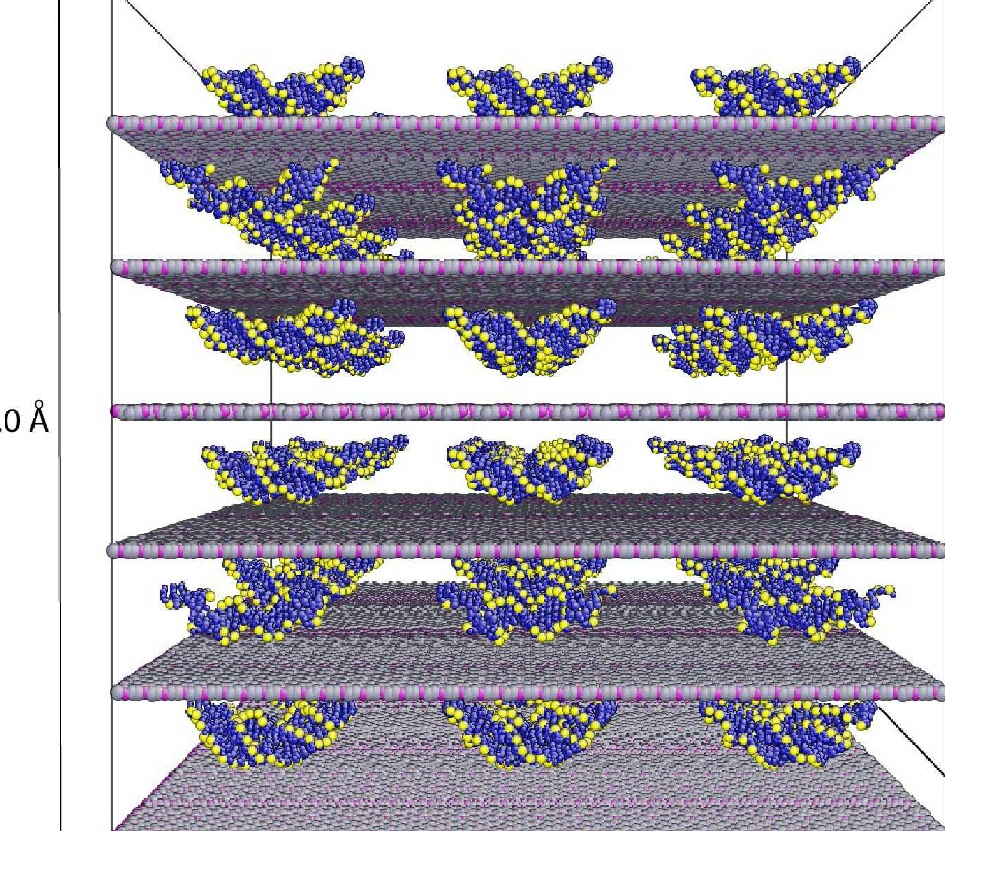
\includegraphics[scale=0.3]{subproject1-bioclays/pic1}
           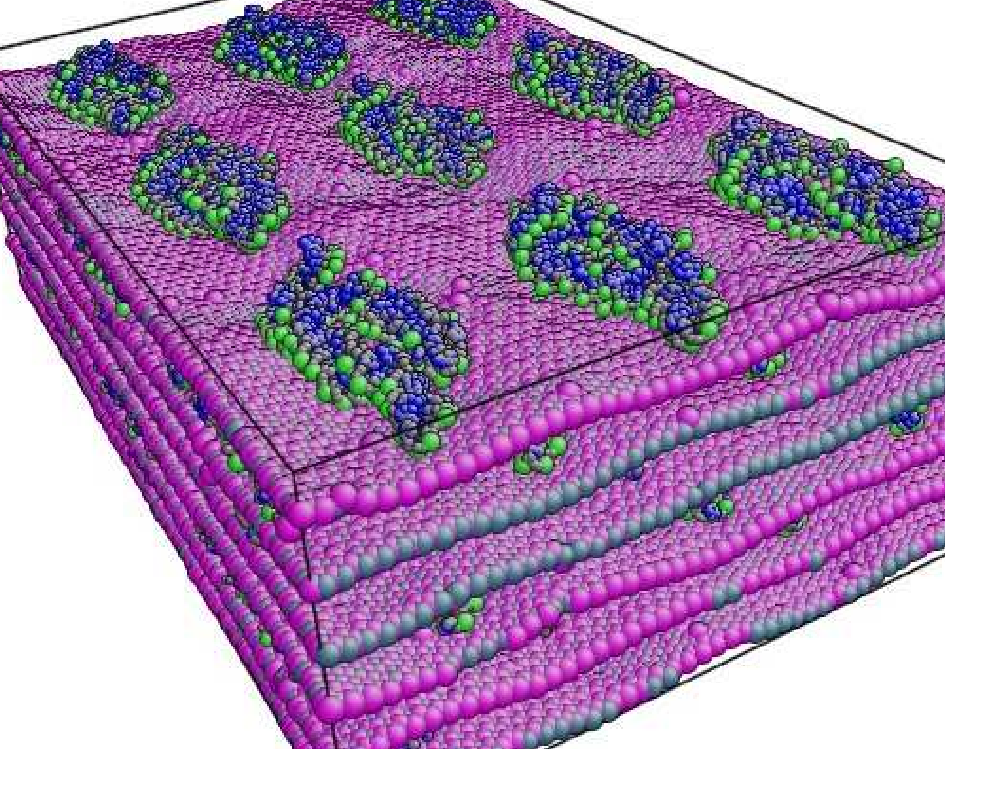
\includegraphics[scale=0.3]{subproject1-bioclays/pic2}
           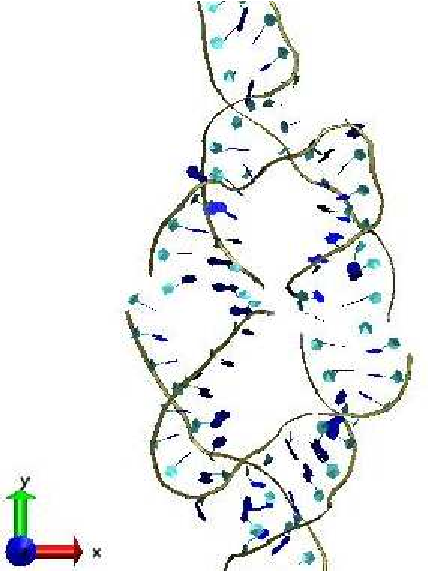
\includegraphics[scale=0.3]{subproject1-bioclays/pic3}
        \end{center}
%\caption{Visualizations of a hammerhead ribozyme intercalated into an LDH clay mineral consisting of 1,181,736 atoms.}
\caption{Initial stucture of the hammerhead ribozyme intercalated into an LDH clay mineral at the 
start of simulation (a) consisting of 1,181,736 atoms.  Magnesium, aluminium, chlorine, phosphorus, 
carbon and nitrogen atoms are represented as light grey, pink, green, yellow, dark grey and blue 
spheres respectively. (b) Final stucture of the large LDH-ribozyme model after the 3.5ns 
production phase of simulation.  Magnesium, aluminium, chlorine, phosphorus, carbon and nitrogen 
atoms are represented as light grey, pink, green, yellow, dark grey and blue spheres respectively.  
All nucleotide motion within the LDH sheets is significantly restricted compared to that in 
bulk water. In addition, visualisation reveals properties such as thermal undulations in the LDH 
sheet, as well as corrugation of the layers around the nucleotides. (c) Visualisation of the ribozyme 
molecule after 3.5ns of simulation, using ribbon notation.}
\label{F:pics}
\end{figure}

%To Each model will include several dispersed ($Na^{+}$ montmorillonite) platelets immersed in either i) a matrix of poly(ethylene glycol) polymer  and ii) large biomolecules such as RNA in aqueous solution. 
%From these simulations will we perform several non-equilbrium molecular dynamics simulations (NEMD), from which we will  calculate material properties, including the bending modulus, Young's
%modulus and Poisson's ratio. %We will also be able to study the interactions between seperate platelets, which may determine the rheology of clay nanocomposites .  It is the increased mechanical and
%thermochemical stability of clay-polymer nanocomposites that has
%received much attention recently in a variety of industries
%\cite{Pinnavaia_book}; 
%our objective is to gain a greater understanding of this enhancement through these
%
%simulations. 
Secondly, we will consider the adsorption of smaller RNA molecules on the edge of clay platelets. 
This will give us insight into the mechanism of
intercalation in these compounds, required for understanding their formation. This is important not just for origins of life studies, but also in the processing conditions for drug delivery applications~\cite{understanding}. For example, we will be able to see changes in the clay sheet conformation that occur with initial intercalation of the bulky biopolymers, such as the layers moving apart from each other, and whether the flexibility of the clay sheet plays a significant role. 

To approach a realistic sized platelet for long simulation times, we require system sizes 
of order 1 - 20 million atoms. The largest system will include several isolated platelets of 
realistic size with biopolymers interacting with the clay sheet edges. This size of simulation 
is now firmly within the mesoscopic regime but simulated in full atomistic detail. We shall 
include non equilibrium simulations to simulate the conditions required for the bulky biopolymers 
to intercalate between the clay sheets on a timescale we can observe with atomistic molecular 
dynamics. These non-equilibrium conditions include compressive stress and shear, which effectively 
force the biopolymers into the clay interlayer region.
%To approach a realistic sized platelet for the long simulation times, we require system sizes of order 1 - 20 million atoms. The largest system will include several isolated platelets of realistic size with biopolymers interacting with the clay sheet edges. This size of simulation is firmly within the `mesoscopic' regime but simulated in full atomistic detail. We shall include non-equilibrium simulations to understand the response of these systems to compressive / extensive stress and under shear. 

%\textbf{Principal scientific objectives} We aim to calculate the
%structural, dynamical and materials properties of a clay platelet
%($Na^{+}$ montmorillonite) immersed in a matrix of poly(ethylene glycol)
%directly from large scale molecular dynamics simulations.
% Additionally  The mechanism of intercalation in clay-polymer
%nanocomposites is unknown, and this will provide valuable
%insight.

%\item\emph{Previous Work on the TeraGrid}
%Publications and progress made in the past year on TG resources.
%In our previous simulations we utilized periodic
%boundaries on the clay sheets, allowing a simulation cell to represent
%an infinite clay platelet \cite{JPCC_2007,Thyveetil,Thyveetil_JACS, Soft_Matter1}.  
%These large-scale, fully atomistic
%simulations, 
%approached the size of a physically realistic platelet.
%From
%this, we were able to calculate mesoscopic and macroscopic properties
%directly from  molecular dynamics simulations in the absence of
%finite-size effects of both clay nanocomposites\cite{JPCC_2007,Thyveetil, Soft_Matter1} and bio-%composites~\cite{Thyveetil_JACS}.

%Using the last LRAC allocation we extended these simulations to calculate 
%the mechanical response of poly(ethylene oxide) polymer-clay nanocomposites, 
%separating the response into contributions from the polymer and clay 
%mineral layer~\cite{Soft_Matter1}. This separation technique allowed us 
%to determine how the clay-polymer elastic properties change with distance 
%from the clay surface. This is the first time the effect of mineral layers 
%on the elastic modulus of polymeric materials in the vicinity of a mineral 
%surface has been calculated. This result is a vital first step to 
%understanding the enhancement mechanism of nanocomposites and the role of 
%the very large surface area of the clay mineral layer on the surrounding medium. To simulate a 
%realistically sized clay platelet required very large scale simulations, made possible using the resources available via 
%the LRAC allocation. 

%We have also examined the mechanisms by which clay mineral layers buckle in clay-polymer nanocomposites under compressive stress. We find that a clay sheet remains stable in a flat state until a critical compressive strain is reached, at which point it buckles, and regains its uncompressed area. Over this buckling transition, the Poisson ratio of the clay sheets turns negative, a property which has been predicted for 2-dimensional sheets ~\cite{Soft_Matter2}. This is the first time such behaviour has been seen in a molecular simulation of mineral layers. The large scale allowing us to probe large buckling wavelengths that are inhibited in smaller scale simulation. 

%We have explicitly included the edges of the clay sheets with the clay platelet completely surrounded by water (Figure~\ref{Fig:water}). The clay platelet consists of  two sheets of $Na^{+}$ montmorillonte clay, which are either aligned or 
%staggered relative to each other in two different models.  
%In long MD simulations, we have observed ingress into the intersheet spacing by water, which is only possible when edges are explicitly included.  We are currently analysing the diffusional properties of the water inside the clay interlayer and the effect on the clay dynamical properties, such as clay sheet thermal undulations. 
%This has never been done before either by simulation or experiment. 
%\begin{figure}
%        \begin{center}
%           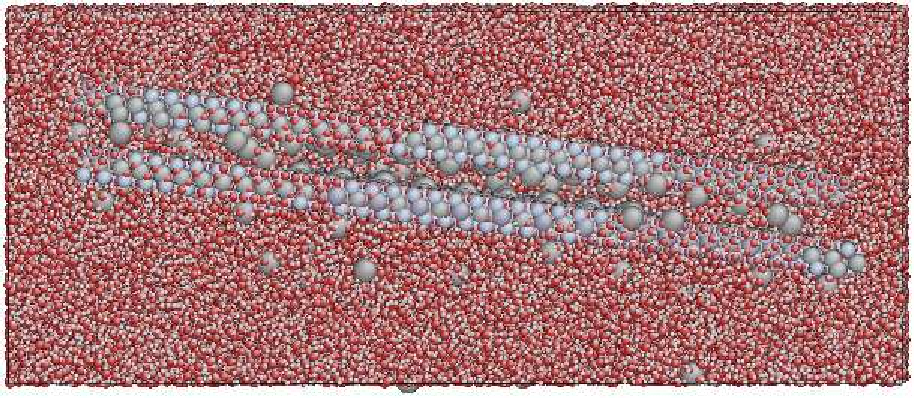
\includegraphics[scale=0.6]{subproject1-bioclays/ymod}
%        \end{center}
%\caption{Visualization of the ingress of water into an isolated clay platelet; the viewpoint is a slice through the clay sheet. Light grey and light blue atoms are the silicon and aluminium atoms of the clay sheet respectively. Oxygen atoms are coloured red and hydrogen atoms are coloured white. Sodium ions, located in the clay interlayer, are dark grey. We can see some sodium ions move away from the surface as the water diffuses through the clay interlayer. }
%\label{Fig:water}
%\end{figure}
% Our previous studies, with periodic boundaries on the clay sheets themselves, were 2/3
%orders of magnitude larger than any previous atomistic simulations of
%clay minerals. They revealed the clay sheets to have some degree of
%flexibility, manifesting as long range, low amplitude undulations with
%wavelengths greater than 25 nm, which are only revealed through
%large scale simulations \cite{jls_2006,thyveetil2007}.  %As an extension 
%to the previous study, we will explicitly include the edges of the 
%clay sheets and the platelet will be completely surrounded by the 
%polymer matrix. The clay platelet will
%consist of  two sheets of $Na^{+}$ montmorillonte clay, which will be
%aligned and staggered relative to each other in two different models.  We
%shall compare the structural and dynamical properties of both the polymer
%and clay platelet to conventional molecular dynamics simulations of
%clay-polymer nanocomposites \cite{cmj_12}.

%\item \emph{Code to be used}
%We will use the scalable molecular dynamics code, LAMMPS \cite{LAMMPS, LAMMPS_2005}, to perform these
%simulations. We will use the rRESPA multi-timestep method \cite{rRESPA} combined with the efficient particle-particle-particle-mesh method \cite{Hockney_book} to calculate the electrostatics. 


%\item \emph{Benchmark Data}
%We have performed comprehensive benchmarks of 
%a hydrated montmorillonite system up to 85 million atoms on Ranger and Kraken.
%See Figure V of the attached `Benchmark Document' for scaling data.

%We find approximately linear scaling up to 2048 processors for 10 million atoms, and up to 4096 for 85 million atoms on Ranger; and up to 2048 for 100 million atoms on Kraken.

\emph{Resource requested:} The simulations to be performed and associated computational requirements are listed in Table \ref{t:claytable}. Each simulation listed of the biopolymer interacting with clay edges will run for 20ns; simulations of the bio-clay systems on the basal clay surfaces will be run for 100ns, to ensure correct conformational sampling of the highly flexible biomolecules is achieved.
 
\begin{table}[!h]
\centering

\begin{tabular}[b]
{|>{\scriptsize}c|>{\scriptsize}c|>{\scriptsize}
c|>{\scriptsize}c|>{\scriptsize}c|>{\scriptsize}c|>{\scriptsize}c|}
\hline
\textbf{Sim Description} & \textbf{No. Sims} &
\textbf{No. Cores} & \textbf{Disk} &
\textbf{Code} & \textbf{TG machine} & \textbf{total SUs}\\
\hline 
Clay edge simulations &  10 & 4096 & 2TB & LAMMPS & Ranger & 2,000,000  \\
\hline
NEMD clay edge simulations & 40 & 4096 & 4TB & LAMMPS & Ranger & 1,000,000 \\
\hline
RNA montmorillonite &  15  & 2048 & 1TB & LAMMPS & Kraken & 500,000 \\
\hline
nucleic-acid LDH & 30 & 2048 & 2TB & LAMMPS & Kraken & 750,000 \\ 
\hline
Grand total of SUs required & & & & & & 4,250,000  \\
\hline
\end{tabular} 
\caption{Summary of biopolymer clay simulations and
simulation times for jobs to be run on Ranger (simulations containing clay edges) and Kraken (interlayer bio-clay composites).}
%\caption{Planned simulations of hydrated
%PEG/$Na^+$-montmorillionite on Ranger 
%(simulations containing clay edges) and Kraken (bio-clay composites).}
\label{t:claytable}
\end{table}
%\end{compactenum}
      


\subsection{Towards patient specific HIV therapy}
%\begin{compactenum}[a)]

\emph{Scientific objectives: } The long term scientific objective of our project is to develop molecular dynamics simulations of HIV-1 Pol enzymes into a tool for clinicians to use in determining the cocktail of drugs to administer to an HIV-infected individual. This work is supported by grants under EU FP7 and FP6 via the VPH-NOE (EU FP7-ICT-2007-5.3 223920), Contra Cancrum (EU FP7-ICT-2007-5.3 223979) and Virolab (EU FP7 223131) projects. For such applications, reproducible accuracy at the level which can rank drug efficacies, and rapidity of acquisition of results (for clinical relevance) are all essential. This takes the application of bio-MD techniques into an entirely new domain.

We have developed an automated protocol to perform simulations and calculate binding affinities in the case of the protease (PR) enzyme\cite{Stoica2008} which we have recently enhanced based on the discovery that ensembles of short simulations produce better sampling than single long timescale simulations\cite{Genheden2009,Sadiq2010}. Molecular dynamics simulations require a crystal structure from which to start, but there will always be far less structures than there are HIV \emph{pol} genotypes. Therefore we need to ensure that we can computationally mutate a crystal structure into any desired 
genotype whilst still accurately calculating binding energy values. Our recent work has successfully reproduced the experimental binding free energy ranking of a series of multiply drug resistant (MDR) mutants of increasing resistance (see Table \ref{tab:mutations}) to the inhibitor lopinavir (LPV) as published by Ohtaka \emph{et al.}\cite{Ohtaka2003}. This selection of six PR sequences will be refered to as the MDR genotype set in the rest of this document. Our next aim is to validate the use of our simulation and analysis protocol by reproducing the results for the other five FDA approved inhibitors included in this study (a list of the inhibitors included is given in Table \ref{tab:inhibitors}).

\begin{table}[h! b! p!]
\begin{center}
\begin{tabular}{ l  l  l }
\textbf{Sequence Code} & \textbf{Description} & \textbf{Mutations}\\
\hline
\textbf{WT} & Wildtype & HXB2\\
\textbf{HM} & MDR hexa-mutant & L10I, M46I, I54V, V82A, I84V, L90M\\
\textbf{QM} & MDR quatro-mutant & M46I, I54V, V82A, I84V\\
\textbf{AS} & Active site mutant & V82A, I84V\\
\textbf{FL} & Flap mutants & M46I, I54V\\
\textbf{DM} & Dimer interface mutants & L10I, L90M\\ 
\hline
\end{tabular}
\end{center}
\caption{Codename and mutational composition of HIV-1 protease sequences investigated.}
\up
\label{tab:mutations}
\end{table}

\begin{table}
\begin{center}
\begin{tabular}{l l}
\textbf{Inhibitor Code} & \textbf{Inhibitor Name}\\
\hline
APV & amprenavir\\
IDV & indinavir\\
LPV & lopinavir\\
NFV & nelfinavir\\
RTV & ritonavir\\
%\textbf{SQV} & \textbf{saquinavir - Better to Remove?}\\
\hline
\end{tabular}
\end{center}
\caption{Code and full names of the HIV-1 protease inhibitors investigated.}
\up\up
\label{tab:inhibitors}
\end{table}

In the last year we have expanded our protocol to include the reverse transcriptase (RT) enzyme and the Non-Nucleotide Reverse Transcriptase Inhibitor (NNRTI) class of drugs for which the required system is more than 3 times larger than PR (solvated RT systems contain 180,000 atoms compared to 50,000 for PR). Our work indicates that the effects of active site mutations can be successfully descriminated using enzyme bound simulations alone (as we do in the protease case), without the need for additional simulations of the apo enzyme. Our intention is to study the inhibitors efavirenz (EFZ) and nevirapine (NVP) bound to wildtype, Y181C, L100I and K103N single mutants, the L100I/Y181C and L100I/K103 double mutants and the L100I/K103N/Y181C triple mutant RT sequences. Our previous work focussed on the L100I and K103N mutations but we have now added the Y181C mutation to this set. Unlike the previous mutations, this gives differing levels of resistance to EFZ and NVP (according to the Stanford database - http://hivdb.stanford.edu/pages/algs/HIVdb.html). Along with calculating the binding free energies of the ligand-bound enzymes, we also intend to extend the individual simulations to investigate the impact of these mutations on the rigid body motions between the fingers and thumb subdomains of the p66 subunit of RT. A recent molecular dynamics study shows that NVP operates as a molecular wedge constraining these catalytically important protein motions\cite{Ivetac2009}. This work indicates that our simulations will need to be of order of at least 30ns in length in order to observe the appropriate properties; along with the evidence from our previous work that free energies calculated for RT simulations vary less than those of PR this informs our decision to perform ensemble-based calculations containing fewer replicas but of longer duration. This second line of investigation provides further justification for including the Y181C mutation as, by replacing the bulky tyrosine residue with the smaller cysteine, a much larger perturbation of the binding pocket geometry is produced which might be expected to invoke more marked alterations in the motions of the fingers and thumb domains.

\emph{Computational Requirements: } We have performed our simulations via the widely used molecular dynamics package NAMD \cite{Phillips2005} with the AMBER \cite{Case2005} suite of MD routines used to parameterise the models prior to simulation and then to analyse the resultant trajectories and calculate the free energy ($\Delta$G) values. In addition to these packages in our future work we plan to use the Nucleic Acid Builder module of AMBER on TeraGrid resources in order to compute the entropy changes via normal mode analysis for the RT system.

Previous work on Ranger benchmarked at 7 hours wallclock time per nanosecond on 32 cores for the protease system and 6.5 hours per nanosecond on 128 cores for reverse transcriptase. These values have been used to estimate the required SUs in Table \ref{t:hiv_req}. We have recently gained access to the Kraken system and have benchmarked the protease system to take 5 hours per nanosecond which, combined with the fast turn-around times, makes Kraken an appealing platform upon which to run our simulations.

The disk requirements for all of the simulations listed in Table \ref{t:hiv_req} will not be required simultaneously; at any
one time it will not exceed 5TB. The majority of this data is *.dcd formatted trajectories output as simulations progress which can be archived once analysis has been completed. The trajectories can be transferred quickly between the TeraGrid and our local storage making use of the optical fibre network infrastructure. We currently have access to 6TB of storage at UCL (UK) and also make extensive use of the Ranch archiving system available at TACC.

\begin{table}[h]
\centering
\begin{tabular}[b]
{|>{\scriptsize}c|>{\scriptsize}c|>{\scriptsize}
c|>{\scriptsize}c|>{\scriptsize}c|>{\scriptsize}c|>{\scriptsize}c|}
\hline
\textbf{Sim Description} & \textbf{No. Sims} &
\textbf{No. Cores} & \textbf{Disk} &
\textbf{Code} & \textbf{TG machine} & \textbf{Total SUs}\\
\hline
\multicolumn{7}{|c|}{\textbf{PR Multiple Drug Resistance Study}}\\
\hline
APV - 6 MDR systems & 400 & 32 & 250GB & NAMD & Ranger & 448,000 \\
\hline
IDV - 6 MDR systems & 400 & 32 & 250GB & NAMD & Ranger & 448,000 \\
\hline
NFV - 6 MDR systems & 400 & 32 & 250GB & NAMD & Ranger & 448,000 \\
\hline
RTV - 6 MDR systems & 400 & 32 & 250GB & NAMD & Ranger & 448,000 \\
\hline
\multicolumn{7}{|c|}{\textbf{RT Drug Resistance Study}}\\
\hline
RT Wildtype EFZ & 10 & 128 & 300GB & NAMD & Kraken & 208,000\\
\hline
RT L100I EFZ & 10 & 128 & 300GB & NAMD & Kraken & 208,000\\
\hline
RT K103N EFZ & 10 & 128 & 300GB & NAMD & Kraken & 208,000\\
\hline
RT Y181C EFZ & 10 & 128 & 300GB & NAMD & Kraken & 208,000\\
\hline
RT L100I/K103N EFZ & 10 & 128 & 300GB & NAMD & Kraken & 208,000\\
\hline
RT L100I/Y181C EFZ & 10 & 128 & 300GB & NAMD & Kraken & 208,000\\
\hline
RT L100I/K103N/Y181C EFZ & 10 & 128 & 300GB & NAMD & Kraken & 208,000\\
\hline
RT Y181C NVP & 10 & 128 & 300GB & NAMD & Kraken & 208,000\\
\hline
RT L100I/Y181C NVP & 10 & 128 & 300GB & NAMD & Kraken & 208,000\\
\hline
RT L100I/K103N/Y181C NVP & 10 & 128 & 300GB & NAMD & Kraken & 208,000\\
\hline
Grand total of SUs required & & & & & & 3,872,000\\
\hline
\end{tabular} \caption{Planned simulations and associated computational requirements.}
\label{t:hiv_req}
\up\up\up
\end{table}
%\end{compactenum}
      


\subsection{Predicting the affinity of the EGFR kinase domain for drug inhibitors of lung cancer}
%\begin{compactenum}[a)]
\emph{Scientific objectives: } The epidermal growth factor receptor (EGFR) is an especially important enzyme target in lung cancer therapy because it mutates and/or is overexpressed in most non-small cell lung carcinoma (NSCLC) tumours. Inhibition of kinase activation of EGFR is a frequently used method to suppress its functions \cite{bib:nature_tki}. The majority of tyrosine kinase inhibitors (TKIs) are ATP-competitive inhibitors which bind in the ATP-binding site. Molecular dynamics (MD) simulations will be used to study the structural and energetic properties of inhibitor-EGFR complexes. The binding affinity of inhibitors to EGFRs will be calculated by molecular mechanics Poisson-Boltzmann surface area (MM/PBSA) methods \cite{bib:wan_philtrans}. This molecular level study is one component of the EU FP7 ContraCancrum (Clinically Oriented Translational Cancer Multilevel Modeling) project which aims at developing a composite multilevel platform for simulating malignant tumor development and pharmacologic responses to a therapeutic intervention (http://www.contracancrum.eu). We have employed large scale MD techniques using both TeraGrid and DEISA resources in order to study the interactions of inhibitors with wild-type and mutant EGFRs \cite{bib:wc2009}. A better understanding of the reasons for the success or failure of a therapeutic intervention will help us in the selection of subgroups of patients who are most likely to respond to specific drugs, and paves the way for personalized treatment \cite{bib:hiv}. We have already performed a preliminary study of different inhibitors (AEE788, AFN941 and gefitinib) with EGFR which we now intend to extend to look at a wider variety of inhibitors and EGFR mutations and to probe longer time scale motions of the protein.

%\item \emph{Benchmark Data}
%\begin{comment}
%\begin{figure}
%\centering
%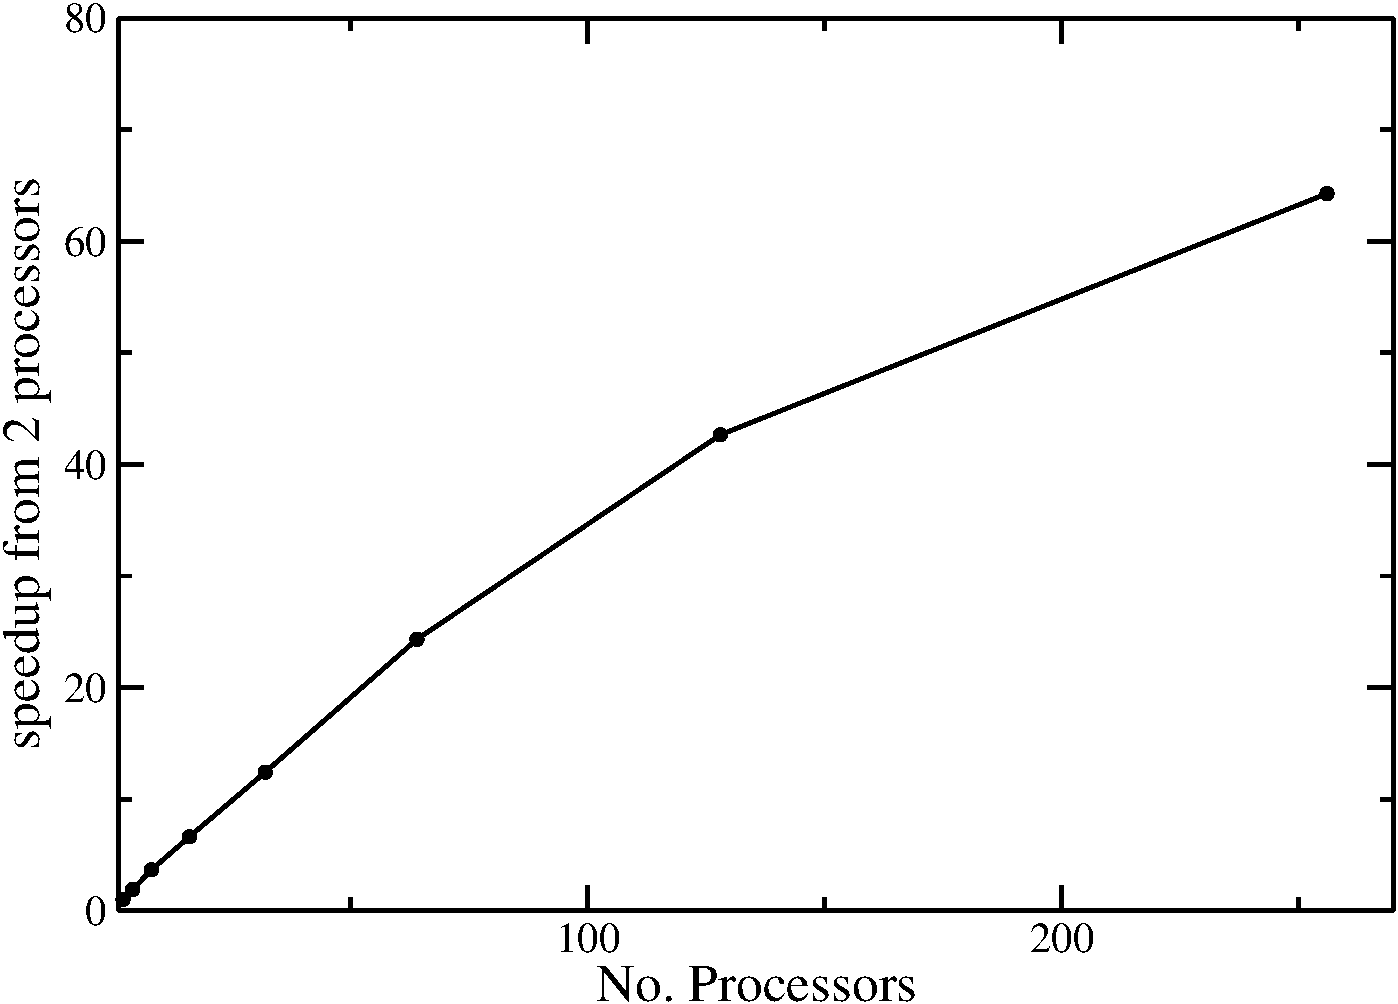
\includegraphics[scale=0.5]{efgr/benchmark}
%\caption{Benchmark of NAMD simulations for inhibitor-EGFR system}\label{fig:benchmark}
%\end{figure}
%\end{comment}
%Based on our benchmark study on Ranger (see Figure VIII of the attached `Benchmark Document'), 
%and preliminary simulations, each simulation will run optimally on 128 processors, 
%and it will consume 300 SUs/ns.
%Based on our benchmark study on Ranger (Figure \ref{fig:benchmark}), and preliminary simulations, each simulation will run optimally on 128 processors, and it will consume about 300 SUs/ns.

\emph{Resource requested:} Computational requirements on Ranger for intended studies of EGFR-inhibitor interaction are listed in Table \ref{t:efgr}.

\begin{table}[h]
\centering
\begin{tabular}[b]
{|>{\scriptsize}c|>{\scriptsize}c|>{\scriptsize}
c|>{\scriptsize}c|>{\scriptsize}c|>{\scriptsize}c|>{\scriptsize}c|}
\hline
\textbf{Sim Description} & \textbf{No. Sims} &
\textbf{No. Cores} & \textbf{Disk} &
\textbf{Code} & \textbf{TG machine} & \textbf{Total SUs}\\
\hline
AEE/EGFRs (50,000 atoms) & 50$^a$ $\times$ 25$^b$ & 128 & 100GB & NAMD & Ranger & 2,000,000\\
\hline
Erlotinib/EGFRs (50,000 atoms) & 5$^c$ $\times$ 50$^a$ $\times$ 1$^b$ & 128 & 100GB & NAMD & Ranger & 400,000\\
\hline
Grand total of SUs required & & & & & & 2,400,000 \\
\hline
\end{tabular} \caption{Planned simulations and associated computational requirements. $^a$Number of replicas in one ensemble simulation; $^b$Number of simulations for each replica, each simulation lasts for 4ns; $^c$Wild-type and 4 mutant (G719S, L858R, T890M and T790M/L858R) EGFRs.}
\label{t:efgr}
\end{table}
%\end{compactenum}


\begin{thebibliography}{10}

\bibitem{zasada2009}
P.~V. Coveney and S.~J. Zasada.
\newblock Virtualizing access to scientific applications with the {Application
  Hosting Environment}.
\newblock {\em Comp. Phys. Comm.}, 180(12):2513--2525, 2009.

\bibitem{coveney2007}
P.~V. Coveney, R.~S. Saksena, S.~J. Zasada, M.~McKeown, and S.~Pickles.
\newblock The application hosting environment: Lightweight middleware for
  grid-based computational science.
\newblock {\em Comp. Phys. Comm.}, 176:406--418, 2007.

\bibitem{chaos-book}
P.~Cvitanovi{\'{c}}, R.~Artuso, R.~Mainieri, G.~Tanner, G.~Vattay, N.~Whelan,
  and A.~Wirzba.
\newblock {\em Chaos: Classical and Quantum (http://www.chaosbook.org/)}.
\newblock Niels Bohr Institute, Copenhagen, 2005.

\bibitem{artuso}
R.~Artuso, E.~Aurell, and P.~Cvitanovi{\'{c}}.
\newblock Recycling of strange sets \uppercase{i}: cycle expansions.
\newblock {\em Nonlinearity}, 3:325--359, 1998.

\bibitem{bohr-jensen}
T.~Bohr, M.~H. Jensen, G.~Paladin, and A.~Vulpiani.
\newblock {\em Dynamical Systems Approach to Turbulence (Cambridge Nonlinear
  Science Series)}.
\newblock Cambridge University Press, 1998.

\bibitem{lan-cvitanovic}
Y.~Lan and P.~Cvitanovi\ifmmode~\acute{c}\else \'{c}\fi{}.
\newblock Variational method for finding periodic orbits in a general flow.
\newblock {\em Phys. Rev. E}, 69(1):016217, 2004.

\bibitem{Comput-HYPO4D}
L.~Fazendeiro, B.~M. Boghosian, P.~V. Coveney, and J.~L{\"{a}}tt.
\newblock Unstable periodic orbits in turbulent hydrodynamics.
\newblock {\em Submitted to the Journal of Computational Science}, 2009.

\bibitem{draft-bogh-tam2}
B.~M. Boghosian, P.~V. Coveney, L.~Fazendeiro, J.~L{\"{a}}tt, J.~Tam, and
  H.~Tang.
\newblock A computational program for the dynamical systems approach to
  turbulence.
\newblock {\em Submitted to Journal of Computational Science}, 2010.

\bibitem{saksenapetascale}
R.~S. Saksena, B.~M. Boghosian, L.~Fazendeiro, O.~A. Kenway, S.~Manos,
  M.~Mazzeo, S.~K. Sadiq, J.~L. Suter, D.~Wright, and P.~V. Coveney.
\newblock Real science at the petascale.
\newblock {\em Phil. Trans. R. Soc. A}, 367(1897):2557--2571, 2009.

\bibitem{viswanath2007}
D.~Viswanath.
\newblock Recurrent motions within plane {Couette} turbulence.
\newblock {\em J. Fluid Mech.}, 580:339--358, 2007.

\bibitem{gibson2008}
J.~F. Gibson, J.~Halcrow, and P.~Cvitanovi\'{c}.
\newblock Visualizing the geometry of state space in plane couette flow.
\newblock {\em J. Fluid Mech.}, 611:107--130, 2008.

\bibitem{dennis1996}
J.~E. Dennis~Jr and R.~B. Schnabel.
\newblock Numerical methods for unconstrained optimization and nonlinear
  equations.
\newblock {\em SIAM}, 1996.

\bibitem{doctors2009}
G.~M. Doctors, M.~D. Mazzeo, and P.~V. Coveney.
\newblock {A computationally efficient method for simulatioon of fluid flow in
  elastic pipes in toand three dimensions}.
\newblock {\em Submitted to Computer Physics Communications}, 2009.

\bibitem{mazzeo2010}
M.~D. Mazzeo, S.~Manos, and P.~V. Coveney.
\newblock {In situ ray tracing and computational steering for interactive blood
  flow simulation}.
\newblock {\em Computer Physics Communications}, 181:355--370, 2010.

\bibitem{manostg08}
S.~Manos, S.~Zasada, M.~D. Mazzeo, R.~Haines, G.~Doctors, S.~Brew, R.~Pinning,
  J.~Brooke, and P.~V. Coveney.
\newblock {Patient specific whole cerebral blood flow simulation: A future role
  in surgical treatment for neurovascular pathologies}.
\newblock {\em Winner of 'Transformational Science Challenge' award at TeraGrid
  2008}, 2008.

\bibitem{manoshpdc08}
S.~Manos, M.~Mazzeo, O.~Kenway, P.~V. Coveney, N.~T. Karonis, and B.~Toonen.
\newblock Distributed {MPI} cross-site run performance using mpig.
\newblock In {\em HPDC '08: Proceedings of the 17th international symposium on
  High performance distributed computing}, pages 229--230, New York, NY, USA,
  2008. ACM.

\bibitem{manosctw08}
S.~Manos, S.~Zasada, and P.~V. Coveney.
\newblock {Life or Death Decision-making: The Medical Case for Large-scale,
  On-demand Grid Computing}.
\newblock {\em CTWatch Quarterly}, 4(1), 2008.

\bibitem{mazzeo2008}
M.~D. Mazzeo and P.~V. Coveney.
\newblock {HemeLB: A high performance parallel lattice-Boltzmann code for large
  scale fluid flow in complex geometries}.
\newblock {\em Computer Physics Communications}, 178(12):894--914, 2008.

\bibitem{saksena2008}
R.~S. Saksena and P.~V. Coveney.
\newblock Self-assembly of ternary cubic, hexagonal, and lamellar mesophases
  using the lattice-{B}oltzmann kinetic method.
\newblock {\em J. Phys. Chem. B}, 112(10):2950 -- 2957, 2008.

\bibitem{harting2004_2}
J.~Harting, Chin. J., M.~Venturoli, and P.~V. Coveney.
\newblock Large-scale grid-enabled lattice-boltzmann simulations of complex
  fluid flow in porous media and under shear.
\newblock {\em Phil. Trans. R. Soc. Lond. A}, 362:1703--1722, 2004.
\newblock there is an updated publication from 2005.

\bibitem{cates2008sm}
M.~E. Cates and P.~S. Clegg.
\newblock Bijels: {A} new class of soft materials.
\newblock {\em Soft Matter}, 4:2132--2138, 2008.

\bibitem{saksena2009_2}
R.~S. Saksena and P.~V. Coveney.
\newblock Shear rheology of amphiphilic cubic liquid crystals from large-scale
  kinetic lattice-boltzmann simulations.
\newblock {\em Soft Matter}, 5:4446--4463, 2009.

\bibitem{saksena1024}
R.~S. Saksena and P.~V. Coveney.
\newblock Defect texture dynamics under couette flow in amphiphilic liquid
  crystals from large-scale lattice-boltzmann simulations. {Preprint} 2010.

\bibitem{saksena2009}
R.~S. Saksena and P.~V. Coveney.
\newblock Rheological response and dynamics of an amphiphilic diamond phase.
\newblock {\em Proc. R. Soc. A}, 465:1977--2002, 2009.

\bibitem{saksenaahm09}
R.~S. Saksena, S.~J. Zasada, M.~D. Mazzeo, and P.~V. Coveney.
\newblock Petascale lattice-{B}oltzmann simulations of amphiphilic cubic liquid
  crystals. {Preprint 2010.}

\bibitem{bmb2005}
B.~M. Boghosian and P.~V. Coveney.
\newblock Scientific applications of grid computing.
\newblock {\em Computing in Science and Engineering}, 7(5):10--13, 2005.

\bibitem{blake-coveney-clarke-pickles-05}
R.~J. Blake, P.~V. Coveney, P.~Clarke, and S.~M. Pickles.
\newblock {\em Scientific Programming}, 13:1--17, 2005.

\bibitem{mckeown_ptrsla05}
R.~Haines, M.~McKeown, S.~M. Pickles, R.~L. Pinning, A.~R. Porter, and
  M.~Riding.
\newblock The service architecture of the teragyrid experiment.
\newblock {\em Phil. Trans. R. Soc. A}, 363:1743--1755, 2005.

\bibitem{hector}
{h}ttp://www.hector.ac.uk.

\bibitem{jens}
Private Communication. {Also see
  {www.hc-europa.eu/files/registrationTAM/6-Florian\%20JANOSCHEK.pdf}}.

\bibitem{JPCC_2007}
J.~L.~Suter \emph{et al}.
\newblock Large-scale molecular dynamics study of montmorillonite clay:
  Emergence of undulatory fluctuations and determination of material
  properties.
\newblock {\em J. Phys. Chem. C}, 111(23):8248--8259, 2007.

\bibitem{Franchi}
M.~Franchi, J.~P. Ferris, and E.~Gallori.
\newblock Cations as mediators of the adsorption of nucleic acids on clay
  surfaces in prebiotic environments.
\newblock {\em {Origins of Life and Evolution of the Biosphere}}, {33}:{1--16},
  {2003}.

\bibitem{Huang}
W. H. Huang and J. P. Ferris.
\newblock One-step, regioselective synthesis of up to 50-mers of {RNA}
  oligomers by montmorillonite catalysis.
\newblock {\em {Journal of the American Chemical Society}}, {128}:{8914--8919},
  {2006}.

\bibitem{understanding}
B.~Chen, J.~R.~G. Evans, H.~C. Greenwell, P.~Boulet, P.~V. Coveney, A.~A.
  Bowden, and A.~Whiting.
\newblock A critical appraisal of polymer-clay nanocomposites.
\newblock {\em Chem. Soc. Rev.}, 37:568--594, 2007.

\bibitem{Thyveetil}
M.-A. Thyveetil, P.~V. Coveney, J.~L. Suter, and H.~C. Greenwell.
\newblock Emergence of undulations and determination of materials properties in
  large-scale molecular dynamics simulation of layered double hydroxides.
\newblock {\em Chem. Mater.}, 19(23):5510--5523, 2007.

\bibitem{Thyveetil_JACS}
M.-A. Thyveetil, P.V. Coveney, H.~C. Greenwell, and J.~L. Suter.
\newblock Computer simulation study of the structural stability and materials
  properties of {DNA}-intercalated layered double hydroxides.
\newblock {\em J. Am. Chem. Soc.}, 130(14):4742--4756, 2008.

\bibitem{Soft_Matter1}
J.~L. Suter and P.~V. Coveney.
\newblock Computer simulation study of the materials properties of intercalated
  and exfoliated poly(ethylene)glycol clay nanocomposites.
\newblock {\em Soft Matter}, 5:2239, 2009.

\bibitem{Soft_Matter2}
J.~L. Suter and P.~V. Coveney.
\newblock Materials properties of clay nanocomposites: onset of negative
  {Poisson} ratio in large-scale molecular dynamics simulation.
\newblock {\em Soft Matter}, 5:3896--3904, 2009.

\bibitem{LAMMPS}
S.~J. Plimpton.
\newblock Fast parallel algorithms for short-range molecular dynamics.
\newblock {\em J. Comp. Phys.}, 117:1--19, 1995.

\bibitem{LAMMPS_2005}
S.~Plimpton.
\newblock Large-scale atomic/molecular massively parallel simulator;
  http://www.cs.sandia.gov/$\sim$sjplimp/lammps.html.
\newblock Sandia National Laboratories, Albuquerque, 2005.

\bibitem{rRESPA}
M.~Tuckerman, B.~J. Berne, and G.~J. Martyna.
\newblock Reversible multiple time scale molecular dynamics.
\newblock {\em J. Chem. Phys.}, 97:1990--2001, 1992.

\bibitem{Hockney_book}
R.~W. Hockney and J.~Eastwood.
\newblock {\em Computer Simulation Using Particles}.
\newblock McGraw-Hill, New York, 1981.

\bibitem{Stoica2008}
I.~Stoica, S.K. Sadiq, and P.V. Coveney.
\newblock Rapid and accurate prediction of binding free energies for
  saquinavir-bound {HIV}-1 proteases.
\newblock {\em Journal of the American Chemical Society}, 130(8):2639--2648,
  2008.

\bibitem{Genheden2009}
S.~Genheden and U.~Ryde.
\newblock How to obtain statistically converged {MM/PBSA} results.
\newblock {\em Journal of Computational Chemistry}, 2009.
\newblock Published online in July 2009.

\bibitem{Sadiq2010}
S.K. Sadiq, D.W. Wright, O.A. Kenway, and P.V. Coveney.
\newblock {Accurate Ensemble Molecular Dynamics Binding Free Energy Ranking of
  Multi-Drug-Resistant HIV-1 Proteases}.
\newblock {\em Journal of Chemical Information and Modelling}, 50(5):890-–905, 2010.

\bibitem{Ohtaka2003}
H.~Ohtaka, A.~Schon, and E.~Freire.
\newblock Multidrug resistance to {HIV-1} protease inhibition requires
  cooperative coupling between distal mutations.
\newblock {\em Biochemistry}, 42(46):13659--13666, Nov 2003.

\bibitem{Ivetac2009}
A.~Ivetac and J.A. McCammon.
\newblock {Elucidating the inhibition mechanism of HIV-1 non-nucleoside reverse
  transcriptase inhibitors through multicopy molecular dynamics simulations.}
\newblock {\em J Mol Biol}, 388(3):644--658, May 2009.

\bibitem{Sadiq2008}
S.~K. Sadiq, M.~D. Mazzeo, S.~J. Zasada, S.~Manos, I.~Stoica, C.~V. Gale, S.~J.
  Watson, P.~Kellam, S.~Brew, and P.~V. Coveney.
\newblock Patient-specific simulation as a basis for clinical decision-making.
\newblock {\em Philosophical Transactions of the Royal Society A: Mathematical,
  Physical and Engineering Sciences}, 366:3199--3219, 2008.

\bibitem{Sadiq2008a}
S.~K. Sadiq, D.~W. Wright, S.~J. Watson, S.~J. Zasada, I.~Stoica, and P.~V.
  Coveney.
\newblock An automated molecular simulation-based binding affinity calculator
  for ligand-bound {HIV}-1 proteases.
\newblock {\em Journal of Chemical Information and Modeling}, 48:1909--1919,
  2008.

\bibitem{Hess2008}
B.~Hess, C.~Kutzner, D.~van~der Spoel, and E.~Lindahl.
\newblock Gromacs 4: Algorithms for highly efficient, load-balanced, and
  scalable molecular simulation.
\newblock {\em Journal of Chemical Theory and Computation}, 4:435--447, 2008.

\bibitem{Phillips2005}
J.~C. Phillips, R.~Braun, W.~Wang, J.~Gumbart, E.~Tajkhorshid, E.~Villa,
  C.~Chipot, R.~D. Skeel, L.~Kale, and K.~Schulten.
\newblock {S}calable molecular dynamics with {NAMD}.
\newblock {\em Journal of Computational Chemistry}, 26(16):1781--1802, Dec
  2005.

\bibitem{Case2005}
D.A. Case, T.E. Cheatham, T.~Darden, H.~Gohlke, R.~Luo, K.M. Merz, A.~Onufriev,
  C~Simmerling, B.~Wang, and R.J. Woods.
\newblock The {A}mber biomolecular simulation programs.
\newblock {\em J Comput Chem}, 26(16):1668--1688, Dec 2005.

\bibitem{bib:nature_tki}
P.~L.~Yang J.~Zhang and N.~S. Gray.
\newblock Targeting cancer with small molecule kinase inhibitors.
\newblock {\em Nat. Rev. Cancer}, 9:28--39, 2009.

\bibitem{bib:wan_philtrans}
S.~Wan, P.~V. Coveney, and D.~R. Flower.
\newblock Peptide recognition by the {T} cell receptor: comparison of binding
  free energies from thermodynamic integration, {Poisson-Boltzmann} and linear
  interaction energy approximations.
\newblock {\em Phil. Trans. R. Soc. Lond. A}, 363(1833):2037--2053, 2005.

\bibitem{bib:wc2009}
S.~Wan and P.~V. Coveney.
\newblock Patient specific prediction of drug binding affinities.
\newblock In {\em The World Congress on Medical Physics and Biomedical
  Engineering, Munich, Germany}, 2009.

\bibitem{bib:hiv}
P.M.A. Sloot, P.V. Coveney, G.~Ertaylan, V.~Mºller, C.A. Boucher, and
  M.~Bubak.
\newblock Hiv decision support: from molecule to man.
\newblock {\em Phil. Trans. R. Soc. A}, 367(1898):2691--2703, 2009.

\bibitem{martin-determination}
H.S.C. Martin, S.~Jha, S.~Howorka, and P.V. Coveney.
\newblock Determination of free energy profiles for the translocation of
  polynucleotides through $\alpha$-hemolysin nanopores using non-equilibrium
  molecular dynamics simulations.
\newblock {\em Journal of Chemical Theory and Computation}, 5(8):33--37, 2009.

\bibitem{henin2004ofe}
J.~H{\'e}nin and C.~Chipot.
\newblock Overcoming free energy barriers using unconstrained molecular
  dynamics simulations.
\newblock {\em The Journal of Chemical Physics}, 121:2904, 2004.

\bibitem{chipot2005exploring}
C.~Chipot and J.~H{\'e}nin.
\newblock Exploring the free-energy landscape of a short peptide using an
  average force.
\newblock {\em Journal of Chemical Physics}, 123:244906, 2005.

\bibitem{Yon1998}
J.~M. Yon, D.~Perahia, and C.~Ghélis.
\newblock Conformational dynamics and enzyme activity.
\newblock {\em Biochimie}, 80(1):33--42, Jan 1998.

\bibitem{Daniel2003}
R.~M. Daniel, R.~V. Dunn, J.~L. Finney, and J.~C. Smith.
\newblock The role of dynamics in enzyme activity.
\newblock {\em Annu Rev Biophys Biomol Struct}, 32:69--92, 2003.

\bibitem{Henzler-Wildman2007}
K.~A. Henzler-Wildman, M.~Lei, V.~Thai, S.~J. Kerns, M.~Karplus, and D.~Kern.
\newblock A hierarchy of timescales in protein dynamics is linked to enzyme
  catalysis.
\newblock {\em Nature}, 450:913--916, 2007.

\bibitem{Nicholson1995}
L.~K. Nicholson, T.~Yamazaki, D.~A. Torchia, S.~Grzesiek, A.~Bax, S.~J. Stahl,
  J.~D. Kaufman, P.~T. Wingfield, P.~Y. Lam, and P.~K. Jadhav.
\newblock Flexibility and function in {HIV-1} protease.
\newblock {\em Nat Struct Biol}, 2(4):274--280, Apr 1995.

\bibitem{Wiley2009}
A.~P. Wiley, S.~L. Williams, and J.~W. Essex.
\newblock {Conformational Motions of HIV-1 Protease Identified Using Reversible
  Digitally Filtered Molecular Dynamics}.
\newblock {\em Journal of Chemical Theory and Computation}, 5:1117--1128, 2009.

\bibitem{Kensch2000}
O.~Kensch, T.~Restle, B.~M. Wöhrl, R.~S. Goody, and H.~J. Steinhoff.
\newblock Temperature-dependent equilibrium between the open and closed
  conformation of the p66 subunit of {HIV-1} reverse transcriptase revealed by
  site-directed spin labelling.
\newblock {\em J Mol Biol}, 301(4):1029--1039, Aug 2000.

\bibitem{Madrid2001}
M.~Madrid, J.~A. Lukin, J.~D. Madura, J.~Ding, and E.~Arnold.
\newblock Molecular dynamics of {HIV-1} reverse transcriptase indicates
  increased flexibility upon dna binding.
\newblock {\em Proteins}, 45(3):176--182, Nov 2001.

\bibitem{Zhou2005}
Z.~Zhou, M.~Madrid, J.~D. Evanseck, and J.~D. Madura.
\newblock Effect of a bound non-nucleoside {RT} inhibitor on the dynamics of
  wild-type and mutant {HIV-1} reverse transcriptase.
\newblock {\em J Am Chem Soc}, 127(49):17253--17260, Dec 2005.

\bibitem{Stone2007}
J.~E. Stone, J.~C. Phillips, P.~L. Freddolino, D.~J. Hardy, L.~G. Trabuco, and
  K.~Schulten.
\newblock Accelerating molecular modeling applications with graphics
  processors.
\newblock {\em Journal of Computational Chemistry}, 28:2618--2640, 2007.

\bibitem{Phillips2009}
J.~C. Phillips and J.~E. Stone.
\newblock Probing biomolecular machines with graphics processors.
\newblock {\em Commun. ACM}, 52(10):34--41, 2009.

\bibitem{kaufman2009}
A.~Kaufman, Z.~Fan, and K.~Petkov.
\newblock Implementing the lattice {Boltzmann} model on commodity graphics
  hardware.
\newblock {\em Journal of Statistical Mechanics: Theory and Experiment},
  2009(06):P06016 (26pp), 2009.

\bibitem{bernaschi2010}
M.~Bernaschi, M.~Fatica, S.~Melchionna, S.~Succi, and E.~Kaxiras.
\newblock A flexible high-performance {Lattice Boltzmann GPU} code for the
  simulations of fluid flows in complex geometries.
\newblock {\em Concurrency Computat.:Pract. Exper.}, 22:1--14, 2010.

\end{thebibliography}



\end{document}


